% \section{The CIS Framework}
% \label{sec:cis}

% \subsection{A two-channel model of the mismatch}
% \label{sec:two_channel}

% \begin{wrapfigure}{r}{0.5\textwidth}
% \vspace{-1.2\baselineskip}
% \centering
% 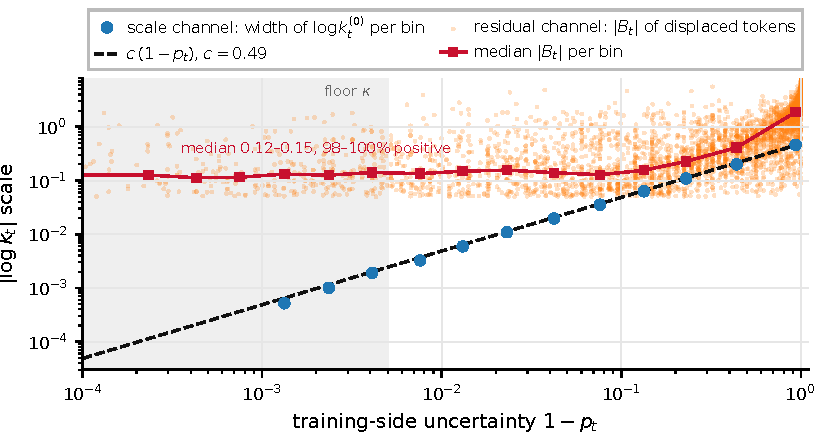
\includegraphics[width=0.5\textwidth]{figures/two_channel.pdf}
% \vspace{-0.6\baselineskip}
% \caption{The two channels on the same tokens (trained MoE policy, 509k tokens). Blue: $|\log k_t|$ when both engines score the same snapshot, and its width per uncertainty bin, which follows $c\,(1-p_t)$ with $c=0.49$ over three decades. Orange: the residual displacement $|B_t|$ on the same tokens, for tokens displaced by more than ten times the storage resolution, and its per-bin median; it stays at $0.12$ to $0.15$ across $1-p_t\in[3\times10^{-4},0.15]$ and is positive on $98$ to $100\%$ of these tokens. The channels overlap only at $1-p_t\gtrsim0.3$; the shaded band is the floor $\kappa$ of \Cref{sec:algorithm}. Details in \Cref{sec:exp_measurement}.}
% \label{fig:two_channel}
% \vspace{-0.8\baselineskip}
% \end{wrapfigure}

% We measured $k_{i,t}$ systematically on large-scale rollouts; experimental
% details are given in \Cref{sec:exp_measurement}. Write
% $p_{i,t}=\pi_{\mathrm{train}}(y_{i,t}\mid x,y_{i,<t};\theta_{\mathrm{old}})$
% for the training-side probability of the token that was actually sampled, and
% drop the index $i$ in what follows. Two facts emerge
% (\Cref{fig:two_channel}). First, the conditional law of $\log k_t$ forms a
% \emph{scale family}, $\log k_t \,\big|\, p_t \overset{d}{=} c\,(1-p_t)\,Z$ with
% the law of $Z$ not depending on $p_t$, so that the shape is fixed and the width
% is proportional to $1-p_t$, where $c>0$ is a constant of the model and engine
% configuration. Second, a small fraction of tokens does not obey this law: their
% deviations do not scale with $1-p_t$, and their magnitude is set by router
% logit gaps and by the storage resolution of the log-probabilities. These two
% facts give the following model.

% \begin{definition}[Two-channel model]
% \label{def:two_channel}
% Conditionally on $p_t$, the observed log-ratio is generated as
% \begin{equation}
% \log k_t
% \;=\;
% c\,(1-p_t)\,Z_t
% \;+\;
% B_t ,
% \label{eq:two_channel}
% \end{equation}
% where the scale component satisfies $Z_t\sim F_Z$ with $F_Z$ independent of
% $p_t$, $\E[Z_t]=0$, $\E|Z_t|<\infty$, $\E[(Z_t)_{+}]>0$, and an upper tail
% that is generalized Pareto with shape $\xi_+\in(0,1)$, no parametric form
% being assumed for $F_Z$; and the residual component satisfies
% $\Prob(B_t\ne0)\le\eps$ and $-B_{\min}\le B_t\le B_{\max}$ with
% $B_{\min},B_{\max}$ independent of $p_t$ on the high-confidence range
% $1-p_t\le\varphi_0$, the event $\{B_t\ne0\}$ being
% independent of $(Z_t,p_t)$ while the value of $B_t$ within the envelope is
% left unmodeled.
% \end{definition}

% \subsection{Estimand and robust risk}
% \label{sec:robust_risk}

% The change of measure $\E[k\,\ell']=\E_{y\sim\pi_{\mathrm{train}}}[\ell']$
% holds exactly; the question is not whether it is valid but which functional of
% the configuration we optimize. The two channels of \Cref{def:two_channel}
% differ on precisely this point. The scale channel is determined by $(c,F_Z)$:
% given a model and an engine configuration it is the same law on every batch.
% The residual channel is determined by which tokens happen to fall on a routing
% boundary or below the storage resolution, and is stable neither across batches
% nor across configurations; carrying it in the target would make the estimand
% move from batch to batch, and no threshold compiled from it would transfer. We
% therefore take the gradient induced by the scale channel alone,
% \begin{equation}
% G_0:=\E\big[e^{\,c(1-p_t)Z_t}\,\ell'\big],
% \label{eq:estimand}
% \end{equation}
% as the estimand; it coincides with $\E[k\,\ell']$ at $\eps=0$, and the residual
% becomes a nuisance---absent from the target, present in every sample.

% For a given sampling law $P$ the mean-squared error of the estimator is
% $\mathcal E_0(\Mclass;P)=\E_P\norm{\widehat G_{\Mclass}-G_0}^{2}$. It cannot be
% optimized directly: $B_t$ is characterized only at the level of sets and
% carries no law to integrate against. We therefore optimize
% \begin{equation}
% \mathcal E(\Mclass)
% :=
% \sup_{P\in\Uset}
% \left\{
% \Big(\sum_p\norm{b_p(\Mclass)}\Big)^{2}
% +\frac{1}{n}\E_P\big[\Mclass^{2}\norm{\ell'}^{2}\big]
% \right\},
% \label{eq:robust_risk}
% \end{equation}
% where
% $b_p(\Mclass)=\E\big[\big(\Mclass(k_t)-e^{\,c(1-p_t)Z_t}\big)\ell'_t\mid p_t=p\big]\,
% \Prob(p_t=p)$
% is the contribution of confidence level $p$ to the bias, and
% $\Uset=\big\{P:\ \log k_t=c(1-p_t)Z_t+B_t,\ Z_t\sim F_Z,\
% \Prob(B_t\ne0)\le\eps,\ -B_{\min}\le B_t\le B_{\max}\big\}$.

% \begin{theorem}[CIS operator, informal]
% \label{thm:cis_informal}
% Under \Cref{def:two_channel}, and when the displacement of the residual channel
% in standardized coordinates is sufficiently large, the minimizer of the robust
% risk over the shrinkage class is
% \begin{equation}
% \log\Mclass^{\star}(k_t,p_t)
% =
% \argminop_{\Mclass\in\Mdown}\mathcal E(\Mclass)
% =
% \min\Big(\log k_t,\;\lambda\,(1-p_t)\Big),
% \label{eq:cis_operator}
% \end{equation}
% where the slope is $\lambda=c\,\tau^{\star}$ and the threshold $\tau^{\star}$
% is uniquely determined by $F_Z$, the residual occurrence rate $\eps$, and the
% sample size $n$.
% \end{theorem}

% \subsection{The deployed algorithm}
% \label{sec:algorithm}

% \Cref{thm:cis_informal} gives a one-sided bound whose width scales with
% $1-p_t$. One correction is needed at the edge of the model's identifiable
% range: as $p_t\to1$ the observed width of $\log k_t$ saturates at the storage
% resolution of the log-probabilities rather than following $c(1-p_t)$, so an
% unfloored band would truncate quantization noise rather than mismatch. We
% therefore floor the scale variable at $\kappa$, which gives \Cref{alg:cis}. The
% two hyperparameters admit measured defaults rather than a search:
% \Cref{thm:cis_informal} compiles $\lambda=c\,\tau^{\star}$, and $\kappa$ is the
% storage resolution of the log-probabilities.

% \begin{wrapfigure}{r}{0.5\textwidth}
% \vspace{-\baselineskip}
% \begin{minipage}{0.5\textwidth}
% \begin{algorithm}[H]
% \caption{Calibrated importance sampling (CIS)}
% \label{alg:cis}
% \begin{algorithmic}[1]
% \Require $\ell^{\mathrm{train}}_j$, $\ell^{\mathrm{infer}}_j$, $\ell'_j$ for
% the $n$ tokens of the batch; $\lambda$; $\kappa$
% \For{$j=1,\dots,n$}
%   \State $\log k_j\gets\ell^{\mathrm{train}}_j-\ell^{\mathrm{infer}}_j$,\quad
%   $p_j\gets\exp(\ell^{\mathrm{train}}_j)$
%   \State $w_j\gets\exp\big(\min\{\log k_j,\;
%   \lambda\max(1-p_j,\kappa)\}\big)$
% \EndFor
% \State \Return $\widehat G_{\mathrm{CIS}}
% =\frac{1}{n}\sum_{j=1}^{n}\operatorname{stopgrad}(w_j)\,\ell'_j$
% \end{algorithmic}
% \end{algorithm}
% \end{minipage}
% \end{wrapfigure}

% The operator adds one elementwise pass and no forward or backward computation.
% Three implementation details are load-bearing: the inference-side
% log-probability must be the raw value recorded at the sampling step, with no
% temperature rescaling or renormalization applied afterwards; the weight must be
% detached, since $k_t$ is data rather than a function of $\theta$; and the floor
% must be applied to $1-p_t$ before multiplication by $\lambda$, not to the
% resulting band.
\section{The CIS Framework}
\label{sec:cis}
\subsection{A logit-displacement model of the mismatch}
\label{sec:logit_model}

\begin{wrapfigure}{r}{0.45\textwidth}
\vspace{-1.2\baselineskip}
\centering
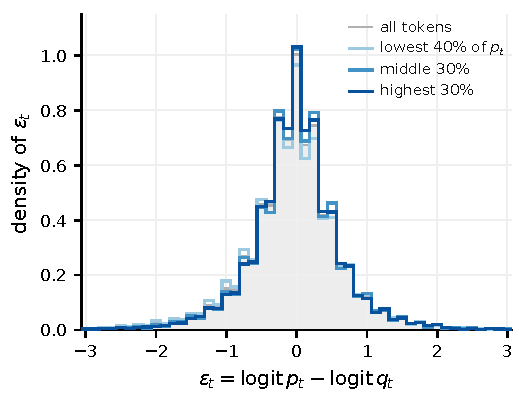
\includegraphics[width=0.45\textwidth]{figures/fig_eps_dist.pdf}
\vspace{-1.4\baselineskip}
\caption{Distribution of $\varepsilon_t$ on a trained MoE, pooled and split by
confidence $p_t$ (histogram bin width $0.125$). The conditional laws coincide.}
\label{fig:eps_dist}
\vspace{-0.8\baselineskip}
\end{wrapfigure}

We measured the pair $(p_t,q_t)$ systematically on large-scale rollouts;
experimental details are given in \Cref{sec:exp_measurement}. Write $p_t=\pi_{\mathrm{train}}(y_t\mid x,y_{<t};\theta_{\mathrm{old}}),
\qquad
q_t=\pi_{\mathrm{infer}}(y_t\mid x,y_{<t};\theta_{\mathrm{old}})$
for the two engines' probabilities of the token that was actually sampled, and
drop the trajectory index $i$ in what follows. The measurements show that the
discrepancy between the two engines is stationary in the log-odds coordinate,
which gives the following model.

\begin{definition}[Logit-displacement model]
\label{def:logit_displacement}
Conditionally on the prefix $h_t$, the two engines' probabilities of the sampled
token satisfy
\begin{equation}
\logit q_t
\;=\;
\logit p_t-\varepsilon_t ,
\qquad
\varepsilon_t\perp p_t ,
\label{eq:logit_displacement}
\end{equation}
where $\mu:=\E[e^{\varepsilon_t}]$ and $\exists\,\alpha>1:\ \E[e^{\alpha\varepsilon_t}]<\infty$.
\end{definition}

Here $\varepsilon_t$ is the log-odds displacement of the inference engine
relative to the training engine on that token, and the substance of the model is
that its distribution does not depend on the confidence.
\Cref{fig:eps_dist} shows the distribution of $\varepsilon_t$, pooled and split
into three confidence groups; a detailed empirical analysis is given in
\Cref{sec:experiments}.

% Solving \eqref{eq:logit_displacement} for the mismatch ratio gives
% \begin{equation}
% k_t
% \;=\;
% p_t+(1-p_t)\,e^{\varepsilon_t}.
% \label{eq:k_geometry}
% \end{equation}
\subsection{Why a correction is needed}
\label{sec:why_correction}

A gradient update uses $n$ tokens (all tokens of all trajectories in the batch).
Write the payload of the $j$-th token as
$\ell'_j=\nabla_\theta\min\big(\rho_j\hat A_j,\operatorname{clip}(\rho_j)\hat A_j\big)$,
the gradient of the surrogate term in \eqref{eq:objective}. Since $k_j$ does not
depend on $\theta$, the gradient of the objective and its $n$-sample estimator
are $G_0:=\nabla_\theta\mathcal J=\E[k\,\ell']$ and
$\widehat G:=\frac{1}{n}\sum_{j=1}^{n}k_j\,\ell'_j$, and we measure the quality
of the estimate by the mean-squared error
$\E\big\|\widehat G-G_0\big\|_2^2$.

\begin{theorem}[Informal]
\label{thm:exact_risk}
Let $k_t$ satisfy \Cref{def:logit_displacement}. Then
\begin{equation}
\E\big\|\widehat G-G_0\big\|_2^2
\;=\;
\frac{1}{n}\Big(c_1+c_2\,\E\big[e^{2\varepsilon_t}\big]\Big),
\label{eq:exact_risk}
\end{equation}
where $c_1,c_2>0$ depend only on the joint law of $(p_t,\ell'_t)$ and not on
$\varepsilon_t$.
\end{theorem}
\begin{wrapfigure}{r}{0.42\textwidth}
\vspace{-1.0\baselineskip}
\centering
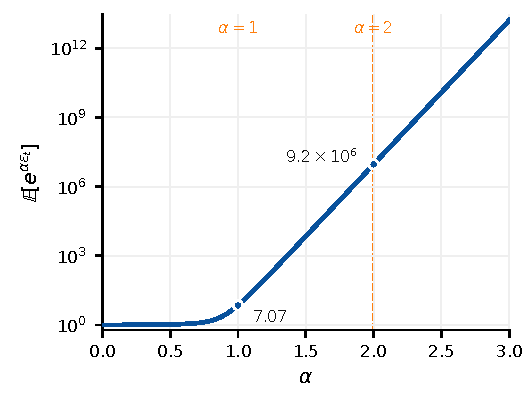
\includegraphics[width=0.42\textwidth]{figures/fig_mgf.pdf}
\vspace{-1.4\baselineskip}
\caption{$\E[e^{\alpha\varepsilon_t}]$ computed from the measured
$\varepsilon_t$.}
\label{fig:mgf}
\vspace{-0.8\baselineskip}
\end{wrapfigure}

\Cref{fig:mgf} shows $\E[e^{\alpha\varepsilon_t}]$ computed from the measured
displacements; details are given in \Cref{app:mgf}. At $\alpha=2$ we obtain
$\E[e^{2\varepsilon_t}]=9.2\times10^{6}$. Our training configuration uses
$n\approx4\times10^{3}$ tokens per update, so the variance term in
\eqref{eq:exact_risk} is of order $10^{3}$.

% One of the reason of this explosive variance is contributed by the explosion of the importance sampling factor $k_j$ when the inference engine and the training engine disagree signficiantly. 
% To mitigate this explosive variance, many existing works introduce some bias in exchane for an well-conditioned variance especially by downweighting the suspicious (overly large) importance sampling factor $k_j$ with the knowledge of it's likelihood $p_j$. Systematically, we can formulate their estimator as ... $\hat G$..

% $\mathcal M -> f(k_j, p_j)$,

% $\hat G_f = 1 / n \sum_{j=1}^n  f(k_j, p_j) \ell_j'$ where $f(k_j, p_j) \in \mathcal F: \{f: 0 \le f(k, p) \le k \}$
% $\hat G_f = 1 / n \sum_{j=1}^n  f(k_j, p_j), where $f(k, j)$ is the corrected importance sampling factor with the liklihood $p_j$ satisfying $f(k, p) \in [0, k]$ implying that $f(k, p)$ cannot exceed the original importance sampling factor. 

We must therefore act on $k_t$. Our objective remains the minimization of
$\E\big\|\widehat G-G_0\big\|_2^2$, and by \Cref{thm:exact_risk} the exact
correction has already driven the bias to zero and placed the entire risk in the
variance; any improvement must come from the opposite direction, by introducing
some bias in exchange for a smaller variance so that their sum is reduced.
Existing token-level corrections do exactly this: TIS caps $k_t$
\citep{cite}, IcePop masks tokens falling outside an interval \citep{cite}, and
KPop masks by a KL threshold \citep{cite}, all of which attenuate a weight but
never amplify it. We write such corrections uniformly as an operator
$\Mclass:(0,\infty)\times(0,1)\to(0,\infty)$ acting on the mismatch ratio, with
estimator


% we note $G_{\mathcal M}$ = \EE M(k_j, p_j) \ell_j'$ where the expectation comes from the randomness of the dataset. 

%\EE [M(k_j, p_j)^2 \cdot \|\ell'\|]
\begin{equation}
\widehat G_{\Mclass}
:=\frac{1}{n}\sum_{j=1}^{n}\Mclass(k_j,p_j)\,\ell'_j ,
\qquad
\Mclass\in\Mdown
:=\big\{\Mclass:\ 0<\Mclass(k,p)\le k\ \ \forall\,(k,p)\big\}.
\label{eq:operator_class}
\end{equation}
The restriction to $\Mdown$ agrees with the methods above and has a reason of
its own: by \eqref{eq:k_geometry} the ratio satisfies $k_t\ge p_t$, so its lower
side is bounded by construction and the variance comes entirely from the upper
side, while amplifying a weight would increase the bias and the variance at
once.
\subsection{The optimal operator}
\label{sec:optimal_operator}

For independent token contributions the mean-squared error of
$\widehat G_{\Mclass}$ admits the upper bound
\begin{equation}
\E\big\|\widehat G_{\Mclass}-G_0\big\|_2^2
\;\le\;
\big\|\E[\Mclass\,\ell']-G_0\big\|_2^2
+\frac{1}{n}\,\E\big[\Mclass^2\|\ell'\|_2^2\big]
\;=:\;
\mathcal R(\Mclass),
\label{eq:surrogate_risk}
\end{equation}
and we take $\mathcal R$ as the surrogate risk and minimize it over the
shrinkage class.

\begin{theorem}[CIS operator, informal]
\label{thm:cis_informal}
Under \Cref{def:logit_displacement},
\begin{equation}
\Mclass^{\star}(k_t,p_t)
=
\argminop_{\Mclass\in\Mdown}\mathcal R(\Mclass)
=
\min\big\{k_t,\;1+\lambda\,(1-p_t)\big\},
\label{eq:cis_operator}
\end{equation}
% absolute constant depends on the momentum of $\varepsilon$, sample size $n$ and the distribution of 
% $\ell'_t$ under distribution $p_t$.
% distribution of $\ell_t$ under $p_t$. 

% $M(x, y) = \alpha x + (1 - \alpha) (1 + \lambda (1 - y))$
% x \le (1 + \lambda (1 - y))
where $\lambda>0$ is uniquely determined by the law of $e^{\varepsilon_t}$, the
sample size $n$, and the joint law of $(p_t,\ell'_t)$.
\end{theorem}

\begin{remark}
\Cref{thm:cis_informal} is an upper bound that tightens with confidence: the
more certain the model is on a token, the closer to one the admissible weight;
the less certain it is, the larger the deviation admitted. On high-confidence
tokens the two engines' probability ratio should already be close to one, so a
large deviation there is more likely to come from numerical noise than from a
genuine difference between the two distributions; on low-confidence tokens the
ratio is dispersed to begin with, and clipping it too tightly discards useful
gradient signal.
\end{remark}

\begin{theorem}[Informal]
\label{thm:cis_risk}
Under the operator of \Cref{thm:cis_informal},
\begin{equation}
\E\big\|\widehat G_{\Mclass^{\star}}-G_0\big\|_2^2
\;\le\;
c_3\,\E\big[(e^{\varepsilon_t}-1-\lambda)_+\big]^2
+\frac{1}{n}\Big(c_1'+c_2\,\E\big[\min(e^{\varepsilon_t},1+\lambda)^2\big]\Big),
\label{eq:cis_risk}
\end{equation}
where $c_2$ is the same constant as in \Cref{thm:exact_risk}, and
$c_1',c_3>0$ likewise depend only on the joint law of $(p_t,\ell'_t)$.
\end{theorem}

\begin{remark}
Compared with \Cref{thm:exact_risk}, the term $\E[e^{2\varepsilon_t}]$ in the
variance is replaced by $\E[\min(e^{\varepsilon_t},1+\lambda)^2]$, which
satisfies
$\E[\min(e^{\varepsilon_t},1+\lambda)^2]\le(1+\lambda)\,\E[e^{\varepsilon_t}]
=(1+\lambda)\,\mu$: the exponent drops from two to one, and the second
exponential moment is traded for the first, which is the constant $\mu$ of
\Cref{def:logit_displacement}, read off \Cref{fig:mgf} at $\alpha=1$ and both
finite and estimable. The price is the bias term, set by the exceedance that the
operator removes and decreasing in $\lambda$.
\end{remark}

\begin{wrapfigure}{r}{0.5\textwidth}
\vspace{-\baselineskip}
\begin{minipage}{0.5\textwidth}
\begin{algorithm}[H]
\caption{Calibrated importance sampling (CIS)}
\label{alg:cis}
\begin{algorithmic}[1]
\Require $\ell^{\mathrm{train}}_j$, $\ell^{\mathrm{infer}}_j$, $\ell'_j$ for
the $n$ tokens of the batch; hyperparameter $\lambda$
\For{$j=1,\dots,n$}
  \State $p_j\gets\exp(\ell^{\mathrm{train}}_j)$,\quad
  $k_j\gets\exp(\ell^{\mathrm{train}}_j-\ell^{\mathrm{infer}}_j)$
  \State $w_j\gets\min\big\{k_j,\;1+\lambda(1-p_j)\big\}$
\EndFor
\State \Return $\widehat G_{\mathrm{CIS}}
=\frac{1}{n}\sum_{j=1}^{n}\operatorname{stopgrad}(w_j)\,\ell'_j$
\end{algorithmic}
\end{algorithm}
\end{minipage}
\end{wrapfigure}

\paragraph{The deployed algorithm.}
The constant $\lambda$ of \Cref{thm:cis_informal} is determined by population
quantities, among them the joint law of $(p_t,\ell'_t)$, which depends on the
training run itself. Rather than estimating these quantities on the fly, our
implementation treats $\lambda$ as a free hyperparameter;
\Cref{sec:exp_hyperparameters} shows that the result is insensitive to it over a
wide range. This gives \Cref{alg:cis}.

The operator adds one elementwise pass and no forward or backward computation.
Two implementation details are load-bearing: the inference-side log-probability
must be the raw value recorded at the sampling step, with no temperature
rescaling or renormalization applied afterwards; and the weight must be
detached, since $k_t$ is data rather than a function of $\theta$.
% \subsection{A two-channel model of the mismatch}
% \label{sec:two_channel}

% % \begin{wrapfigure}{r}{0.5\textwidth}
% % \vspace{-1.2\baselineskip}
% % \centering
% % 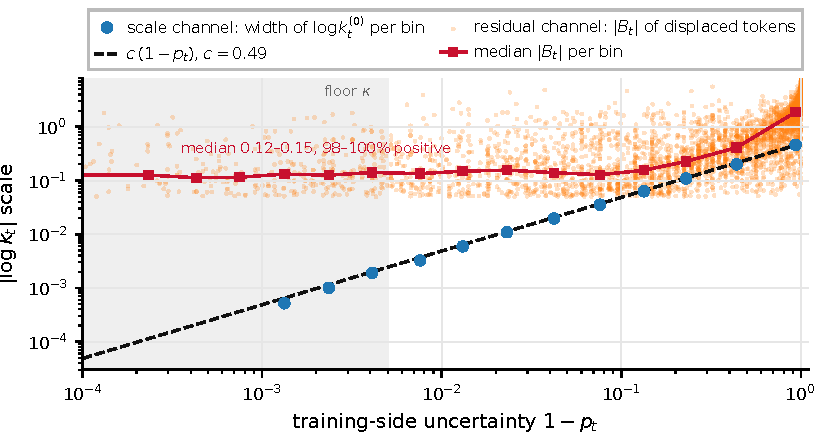
\includegraphics[width=0.5\textwidth]{figures/two_channel.pdf}
% % \vspace{-0.6\baselineskip}
% % \caption{Two channels on the same tokens (trained MoE, 509k tokens): the scale channel $|\log k_t|$ (blue) has width $\propto 1-p_t$; the residual $|B_t|$ (orange) does not scale and is almost entirely positive. Shaded: the floor $\kappa$. Details in \Cref{sec:exp_measurement}.}
% % \label{fig:two_channel}
% % \vspace{-0.8\baselineskip}
% % \end{wrapfigure}

% We measured $k_{i,t}$ systematically on large-scale rollouts; experimental
% details are given in \Cref{sec:exp_measurement}. Write
% $p_{i,t}=\pi_{\mathrm{train}}(y_{i,t}\mid x,y_{i,<t};\theta_{\mathrm{old}})$
% for the training-side probability of the token that was actually sampled, and
% drop the index $i$ in what follows. Two facts emerge
% (\Cref{fig:two_channel}). First, the conditional law of $\log k_t$ forms a
% \emph{scale family}, $\log k_t \,\big|\, p_t \overset{d}{=} c\,(1-p_t)\,Z$ with
% the law of $Z$ not depending on $p_t$, so that the shape is fixed and the width
% is proportional to $1-p_t$, where $c>0$ is a constant of the model and engine
% configuration. Second, a small fraction of tokens does not obey this law: their
% deviations do not scale with $1-p_t$, and their magnitude is set by router
% logit gaps and by the storage resolution of the log-probabilities. These two
% facts give the following model.

% \begin{definition}[Two-channel model]
% \label{def:two_channel}
% Conditionally on $p_t$, the observed log-ratio is generated as
% \begin{equation}
% \log k_t
% \;=\;
% c\,(1-p_t)\,Z_t
% \;+\;
% B_t ,
% \label{eq:two_channel}
% \end{equation}
% where the two components satisfy the following.

% \emph{(i) Scale component.} $Z_t\sim F_Z$ with $F_Z$ independent of $p_t$, and
% \begin{equation}
% \E[Z_t]=0,
% \qquad
% \E\abs{Z_t}<\infty,
% \qquad
% \E[(Z_t)_+]>0,
% \qquad
% z_{\min}(p_t)\le Z_t\le z_{\max}(p_t),
% \label{eq:scale_conditions}
% \end{equation}
% the endpoints of the support being induced by the constraint
% $p_t\le k_t\le 1/\pi_{\mathrm{infer}}(y_t)$. Beyond an upper tail that is
% generalized Pareto with shape $\xi_+\in(0,1)$ within that support, no
% parametric form is assumed for $F_Z$.

% \emph{(ii) Residual component.} $\Prob(B_t\ne0)\le\eps$, the event
% $\{B_t\ne0\}$ is independent of $(Z_t,p_t)$, and
% \begin{equation}
% -B_{\min}\le B_t\le B_{\max},
% \qquad
% B_{\min},B_{\max}\ \text{independent of}\ p_t;
% \qquad
% B_t\ge0
% \ \ \text{when}\ \
% 1-p_t\le\varphi_0 .
% \label{eq:residual_conditions}
% \end{equation}
% The value of $B_t$ within the envelope is left unmodeled.
% \end{definition}

% \subsection{Estimand and robust risk}
% \label{sec:robust_risk}

% The per-step change of measure
% $\E[k_t\,\ell'_t\mid h_t]=\E_{y_t\sim\pi_{\mathrm{train}}}[\ell'_t\mid h_t]$
% holds exactly at every prefix $h_t$; the question is not whether it is valid
% but which functional of the configuration we optimize. The two channels of
% \Cref{def:two_channel} differ on precisely this point. The scale channel is
% determined by $(c,F_Z)$: given a model and an engine configuration it is the
% same law on every batch. The residual channel is determined by which tokens
% happen to fall on a routing boundary or below the storage resolution, and is
% stable neither across batches nor across configurations; carrying it in the
% target would make the estimand move from batch to batch, and no threshold
% compiled from it would transfer. We therefore take the gradient induced by the
% scale channel alone,
% \begin{equation}
% G_0:=\E\big[e^{\,c(1-p_t)Z_t}\,\ell'\big],
% \label{eq:estimand}
% \end{equation}
% as the estimand; it coincides with $\E[k\,\ell']$ at $\eps=0$, and the residual
% becomes a nuisance---absent from the target, present in every sample.

% For a given sampling law $P$ the mean-squared error of the estimator is
% $\mathcal E_0(\Mclass;P)=\E_P\norm{\widehat G_{\Mclass}-G_0}^{2}$. It cannot be
% optimized directly: $B_t$ is characterized only at the level of sets and
% carries no law to integrate against. We therefore optimize
% \begin{equation}
% \mathcal E(\Mclass)
% :=
% \sup_{P\in\Uset}
% \left\{
% \Big(\sum_p\norm{b_p(\Mclass)}\Big)^{2}
% +\frac{1}{n}\E_P\big[\Mclass^{2}\norm{\ell'}^{2}\big]
% \right\},
% \label{eq:robust_risk}
% \end{equation}
% where
% $b_p(\Mclass)=\E\big[\big(\Mclass(k_t)-e^{\,c(1-p_t)Z_t}\big)\ell'_t\mid p_t=p\big]\,
% \Prob(p_t=p)$
% is the contribution of confidence level $p$ to the bias, and
% $\Uset=\big\{P:\ \log k_t=c(1-p_t)Z_t+B_t,\ Z_t\sim F_Z,\
% \Prob(B_t\ne0)\le\eps,\ -B_{\min}\le B_t\le B_{\max}\big\}$.

% \begin{theorem}[CIS operator, informal]
% \label{thm:cis_informal}
% Under \Cref{def:two_channel}, and when the displacement of the residual channel
% in standardized coordinates is sufficiently large, to first order on the log
% scale the minimizer of the robust risk over the shrinkage class is
% \begin{equation}
% \log\Mclass^{\star}(k_t,p_t)
% =
% \argminop_{\Mclass\in\Mdown}\mathcal E(\Mclass)
% =
% \min\Big(\log k_t,\;\lambda\,(1-p_t)\Big),
% \label{eq:cis_operator}
% \end{equation}
% where the slope is $\lambda=c\,\tau^{\star}$ and the threshold $\tau^{\star}$
% is uniquely determined by $F_Z$, the residual occurrence rate $\eps$, and the
% sample size $n$.
% \end{theorem}

% \subsection{The deployed algorithm}
% \label{sec:algorithm}

% \Cref{thm:cis_informal} gives a one-sided bound whose width scales with
% $1-p_t$. One correction is needed once $c(1-p_t)$ falls below the storage
% resolution of the log-probabilities: there the observed width of $\log k_t$
% saturates at that resolution rather than following $c(1-p_t)$, the two
% components of \eqref{eq:two_channel} cannot be separated in the data, and an
% unfloored band would truncate quantization noise rather than mismatch. We
% therefore floor the scale variable at $\kappa$, which gives \Cref{alg:cis}.
% The two hyperparameters admit measured defaults rather than a search:
% \Cref{thm:cis_informal} compiles $\lambda=c\,\tau^{\star}$, and $\kappa$ is the
% storage resolution of the log-probabilities.

% \begin{wrapfigure}{r}{0.5\textwidth}
% \vspace{-\baselineskip}
% \begin{minipage}{0.5\textwidth}
% \begin{algorithm}[H]
% \caption{Calibrated importance sampling (CIS)}
% \label{alg:cis}
% \begin{algorithmic}[1]
% \Require $\ell^{\mathrm{train}}_j$, $\ell^{\mathrm{infer}}_j$, $\ell'_j$ for
% the $n$ tokens of the batch; $\lambda$; $\kappa$
% \For{$j=1,\dots,n$}
%   \State $\log k_j\gets\ell^{\mathrm{train}}_j-\ell^{\mathrm{infer}}_j$,\quad
%   $p_j\gets\exp(\ell^{\mathrm{train}}_j)$
%   \State $w_j\gets\exp\big(\min\{\log k_j,\;
%   \lambda\max(1-p_j,\kappa)\}\big)$
% \EndFor
% \State \Return $\widehat G_{\mathrm{CIS}}
% =\frac{1}{n}\sum_{j=1}^{n}\operatorname{stopgrad}(w_j)\,\ell'_j$
% \end{algorithmic}
% \end{algorithm}
% \end{minipage}
% \end{wrapfigure}

% The operator adds one elementwise pass and no forward or backward computation.
% Three implementation details are load-bearing: the inference-side
% log-probability must be the raw value recorded at the sampling step, with no
% temperature rescaling or renormalization applied afterwards; the weight must be
% detached, since $k_t$ is data rather than a function of $\theta$; and the floor
% must be applied to $1-p_t$ before multiplication by $\lambda$, not to the
% resulting band.